\clearpage % clear the prior chapter's page

\chapter{Rapid simulation of unprocessed DEER decay data for protein fold prediction}\label{ch:rosettadeer}
%\vspace{-7mm}
%\bigskip

The contents of this chapter have been previously published \citep*{DelAlamo2020}.

\bigskip

Despite advances in sampling and scoring strategies, Monte Carlo modeling methods still struggle to accurately predict \emph{de novo} the structures of large proteins, membrane proteins, or proteins of complex topologies. Previous approaches have addressed these shortcomings by leveraging sparse distance data gathered using \gls{sdsl} and \gls{epr} spectroscopy to improve protein structure prediction and refinement outcomes. However, existing computational implementations entail compromises between coarse-grained models of the spin label that lower the resolution and explicit models that lead to resource-intense simulations. These methods are further limited by their reliance on distance distributions, which are calculated from a primary refocused echo decay signal and contain uncertainties that may require manual refinement. Here, we addressed these challenges by developing RosettaDEER, a scoring method within the Rosetta software suite capable of simulating \gls{deer} distance distributions and decay traces between spin labels fast enough to fold proteins \emph{de novo}. We demonstrate that the accuracy of resulting distance distributions match or exceed those generated by more computationally intensive methods. Moreover, decay traces generated from these distributions recapitulate intermolecular background coupling parameters, even when the time window of \gls{epr} data collection is truncated. As a result, RosettaDEER can discriminate between poorly folded and native-like models using decay traces that cannot be accurately converted into distance distributions using regularized fitting approaches. Finally, using two challenging test cases, we demonstrate that RosettaDEER leverages these experimental data for protein fold prediction more effectively than previous methods. These benchmarking results confirm that RosettaDEER can effectively leverage sparse experimental data for a wide array of modeling applications built into the Rosetta software suite.

\section{Introduction}

Structural biology increasingly relies on integrated methods to model the structure and dynamics of proteins and protein assemblies \citep*{Steven2008, Xia2017}. Multiple complementary experimental methodologies can describe the structure and dynamics of proteins that elude determination from a single technique, such as integral membrane proteins, conformationally flexible proteins, and those that fall outside the size limitations of solution-state nuclear magnetic resonance and \gls{cryoem}. By integrating experimental data from multiple approaches, computational modeling can build accurate models in regions with sparse experimental data. One promising source of high-resolution experimental data for integrated structural biology combines \gls{sdsl} and \gls{epr} \citep*{Jeschke2018a, Sahu2018}. Previous studies have employed \gls{sdsl}-\gls{epr} and computation in tandem to predict protein structures \emph{de novo} \citep*{Alexander2008, Fischer2015, Fischer2017, Fischer2016, Hirst2011, Kazmier2011, Ling2016, Yang2010}, model conformational changes \citep*{Kazmier2014, Kazmier2014a, Marinelli2019, Raghuraman2014}, and dock rigid-bodies \citep*{ Bhatnagar2007, Edwards2014, Hilger2007}.

Existing modeling methods largely focus on data gathered using four-pulse \gls{deer} \citep*{Pannier2000}, which can report on distances of up to \SIrange{60}{80}{\angstrom} between stable unpaired electrons conjugated to the protein backbone by \gls{sdsl} \citep*{Jeschke2012, Mchaourab2011}. However, incorporation of these distances as interatomic restraints for modeling purposes is confounded by the conformational freedom of these paramagnetic probes. The central challenge is to convert inter-spin distance information into structural restraints that report on the protein backbone \citep*{Abdullin2016, Alexander2014, Iwahara2004}. Additionally, the need to incorporate two spin labels into the protein sequence per restraint results in sparse coverage of the experimental data that can introduce ambiguities into computational modeling \citep*{Kazmier2011}. As a result, only a few experimental restraints are generally available to describe the protein fold.

These sparse datasets have nonetheless been leveraged for protein structure prediction and refinement by a range of computational modeling approaches that represent the spin labels either implicitly or explicitly. Implicit models such as the \gls{cone} model \citep*{Alexander2008} use knowledge-based potentials to translate inter-spin distance values into backbone restraints, typically between $\mathrm{C_{\upbeta}}$ atoms \citep*{Sale2005}. Introducing these restraints led to measurable improvements in \emph{de novo} structure prediction benchmarks by programs employing Monte Carlo sampling strategies \citep*{Alexander2008, Fischer2015, Fischer2017, Fischer2016, Hirst2011, Kazmier2011}, gradient minimization \citep*{Ling2016, Yang2010}, and molecular dynamics \citep*{MacCallum2015}. However, because these potentials fail to account for the environment or the relative orientations of the spin labels, they tend to be ambiguous \citep*{Sale2005}. Explicit methods, by contrast, model spin labels as either individual side chains \citep*{Alexander2013, Dastvan2016, Krug2016,  Marinelli2019, Marinelli2015}, ensembles of side chains \citep*{Hagelueken2012, Hatmal2012, Hilger2007, Polyhach2011}, or ensembles of dummy atoms \citep*{Islam2013, Kazmier2014, Kazmier2014a}. The added detail improves accuracy of modeling but makes implementations too computationally intensive for \emph{de novo} protein structure prediction and limits the utility of these methods to modeling small-scale conformational changes \citep*{Kazmier2014, Kazmier2014a, Marinelli2019}.

Despite their diversity, these methods largely share a common limitation in their reliance on distance distributions, rather than the primary spectroscopic readout. Other computational methodologies directly incorporate primary experimental data, such as two-dimensional NMR spectr \citep*{Meiler2003} and \gls{cryoem} electron density maps \citep*{Wang2016} to fold and refine proteins. The feasibility of using \gls{deer} dipolar coupling decay traces as modeling restraints has only recently been explored \citep*{Marinelli2019}. Whereas processing spectroscopic decay traces into distance distributions risks introducing ambiguities and artifacts \citep*{Brandon2012, Hustedt2018, Jeschke2006, K.IlkerSen2007, Worswick2018}, simulating a decay trace from a distance distribution is well-described and mathematically straightforward \citep*{Hogben2011, Hustedt2018, Jeschke2012, Marinelli2019}.

Here we introduce RosettaDEER, a method in the macromolecular modeling suite Rosetta capable of rapidly simulating distance distributions and \gls{deer} decay traces between spin labels as well as evaluating a model’s agreement with experimental data. RosettaDEER’s computational efficiency enables prediction of protein structures \emph{de novo} with greater accuracy than the default energy function or the CONE model. Owing to Rosetta’s Monte Carlo sampling strategy \citep*{Leaver-fay2011}, the experimental data can be used directly without analysis or background-correction. Thus, as with other forward modeling approaches\citep*{Stein2015}, the quality of the primary spectroscopic data can be significantly poorer than what would ordinarily be required for rigorous transformation into distance distributions using common fitting strategies. This method reinforces the utility of \gls{deer} in conjunction with computational modeling to accurately model protein structures.

\section{Materials and Methods}\label{sec:rosettadeer_methods}

\subsection{Assembly of diverse experimental datasets}

RosettaDEER was implemented in the Rosetta software suite \citep*{Leaver-fay2011, Leman2020}, trained on distance data gathered in T4 Lysozyme obtained from the laboratory of Hassane S. Mchaourab, and tested and cross-validated using both raw spectroscopic and analyzed distance data gathered in five laboratories (Table \ref{tab:rosettadeer_main_proteins}). Data for the ExoU C-terminus \citep*{Fischer2017}, Bax \citep*{Bleicken2014}, and Mhp1 \citep*{Kazmier2014a} were obtained from and analyzed by the laboratories of Dr. Jimmy Feix, Dr. Enrica Bordignon, and Dr. Hassane S. Mchaourab, respectively. New ExoU double-cysteine mutants were purified, spin labeled, measured and analyzed as previously described (Figure \ref{fig:rosettadeer_supp_exou}) \citep*{Fischer2017}. Raw data for CDB3 \citep*{Zhou2005} and bovine rhodopsin \citep*{Altenbach2008} were obtained from the laboratories of Dr. Albert Beth and Dr. Wayne Hubbell, respectively, and were analyzed using DEERAnalysis2016 \citep*{Jeschke2006}; the last \SI{200}{ns} and \SI{500}{ns} were removed from experimental decay traces shorter and longer than \SI{1.5}{\upmu s}, respectively. The distribution of restraints is shown in Figure \ref{fig:rosettadeer_supp_restraints}.

\subsection{Generation of DEER distance distributions}

The accuracy of various methods that simulate distance distributions between spin labels were compared using Bax (PDB: 1F16, NMR state 8), ExoU (PDB: 3TU3), CDB3 (PDB: 1HYN chains R/S), Rhodopsin (PDB: 1GZM chain A), and Mhp1 (PDB: 2JLN). The methods compared were MMM \citep*{Polyhach2011}, MDDS \citep*{Islam2013}, MtsslWizard \citep*{Hagelueken2012}, Pronox \citep*{Hatmal2012}, and TagDock \citep*{Edwards2014} (See Figure \ref{fig:rosettadeer_main_pseudorotamer} and Table \ref{tab:rosettadeer_main_proteins}). MMM2017 was run locally on both cryogenic \SI{175}{K} and ambient mode \SI{298}{K} with default settings. MDDS was run using the CHARMM-GUI web server \citep*{Jo2014}. MtsslWizard was run locally from PyMol 1.7.2.1 using tight fitting unless no rotamers could be placed, in which case loose fitting was used (Mhp1 residue 324 could not be labeled using loose fitting). Pronox was run from the USC web server using a bias of 0.9 and a van der Waals radius scaling factor of 0.75, the latter of which was reduced to 0.4 if rotamers could not be placed. TagDock was run locally with SCWRL4 \citep*{Krivov2009} and a bump radius of 0.85. Measurements using the CONE model \citep*{Alexander2008, Hirst2011} were determined by adding \SI{1.79}{\angstrom} to the $\mathrm{C_{\upbeta}}$-$\mathrm{C_{\upbeta}}$ distance.

\begin{wraptable}{R}{0.7\textwidth}
\scriptsize
\renewcommand{\tabcolsep}{0.15cm}
\centering
\caption[Benchmark set for the evaluation of RosettaDEER.]{Benchmark set for the evaluation of RosettaDEER.}

\newcolumntype{Y}{>{\raggedright\arraybackslash}X}

\begin{center}
\begin{tabular}{l l l l l}
\toprule \\
 \textbf{Protein} & \textbf{Organism} & \textbf{Restraints} & \textbf{PDB ID} & \textbf{Reference}  \\ \\
\midrule \\
Bax & \emph{Homo sapiens} & 21 & PDB: 1F16 model 8 & \citep*{Bleicken2014}  \\ 
ExoU & \emph{Pseudomonas aeruginosa} & 11 & PDB: 3TU3 & \citep*{Fischer2017} \\
CDB3 & \emph{Homo sapiens} & 15 & PDB: 1HYN R/S & \citep*{Zhou2005} \\
Rhodopsin & \emph{Bos taurus} & 14 & PDB: 1GZM A & \citep*{Altenbach2008} \\
Mhp1 & \emph{Microbacterium tumefaciens} & 18 & PDB: 2JLN & \citep*{Weyand2008} \\

\bottomrule \\
\end{tabular} 
\end{center}




\label{tab:rosettadeer_main_proteins}
\end{wraptable}

\begin{figure}[h]
\centering
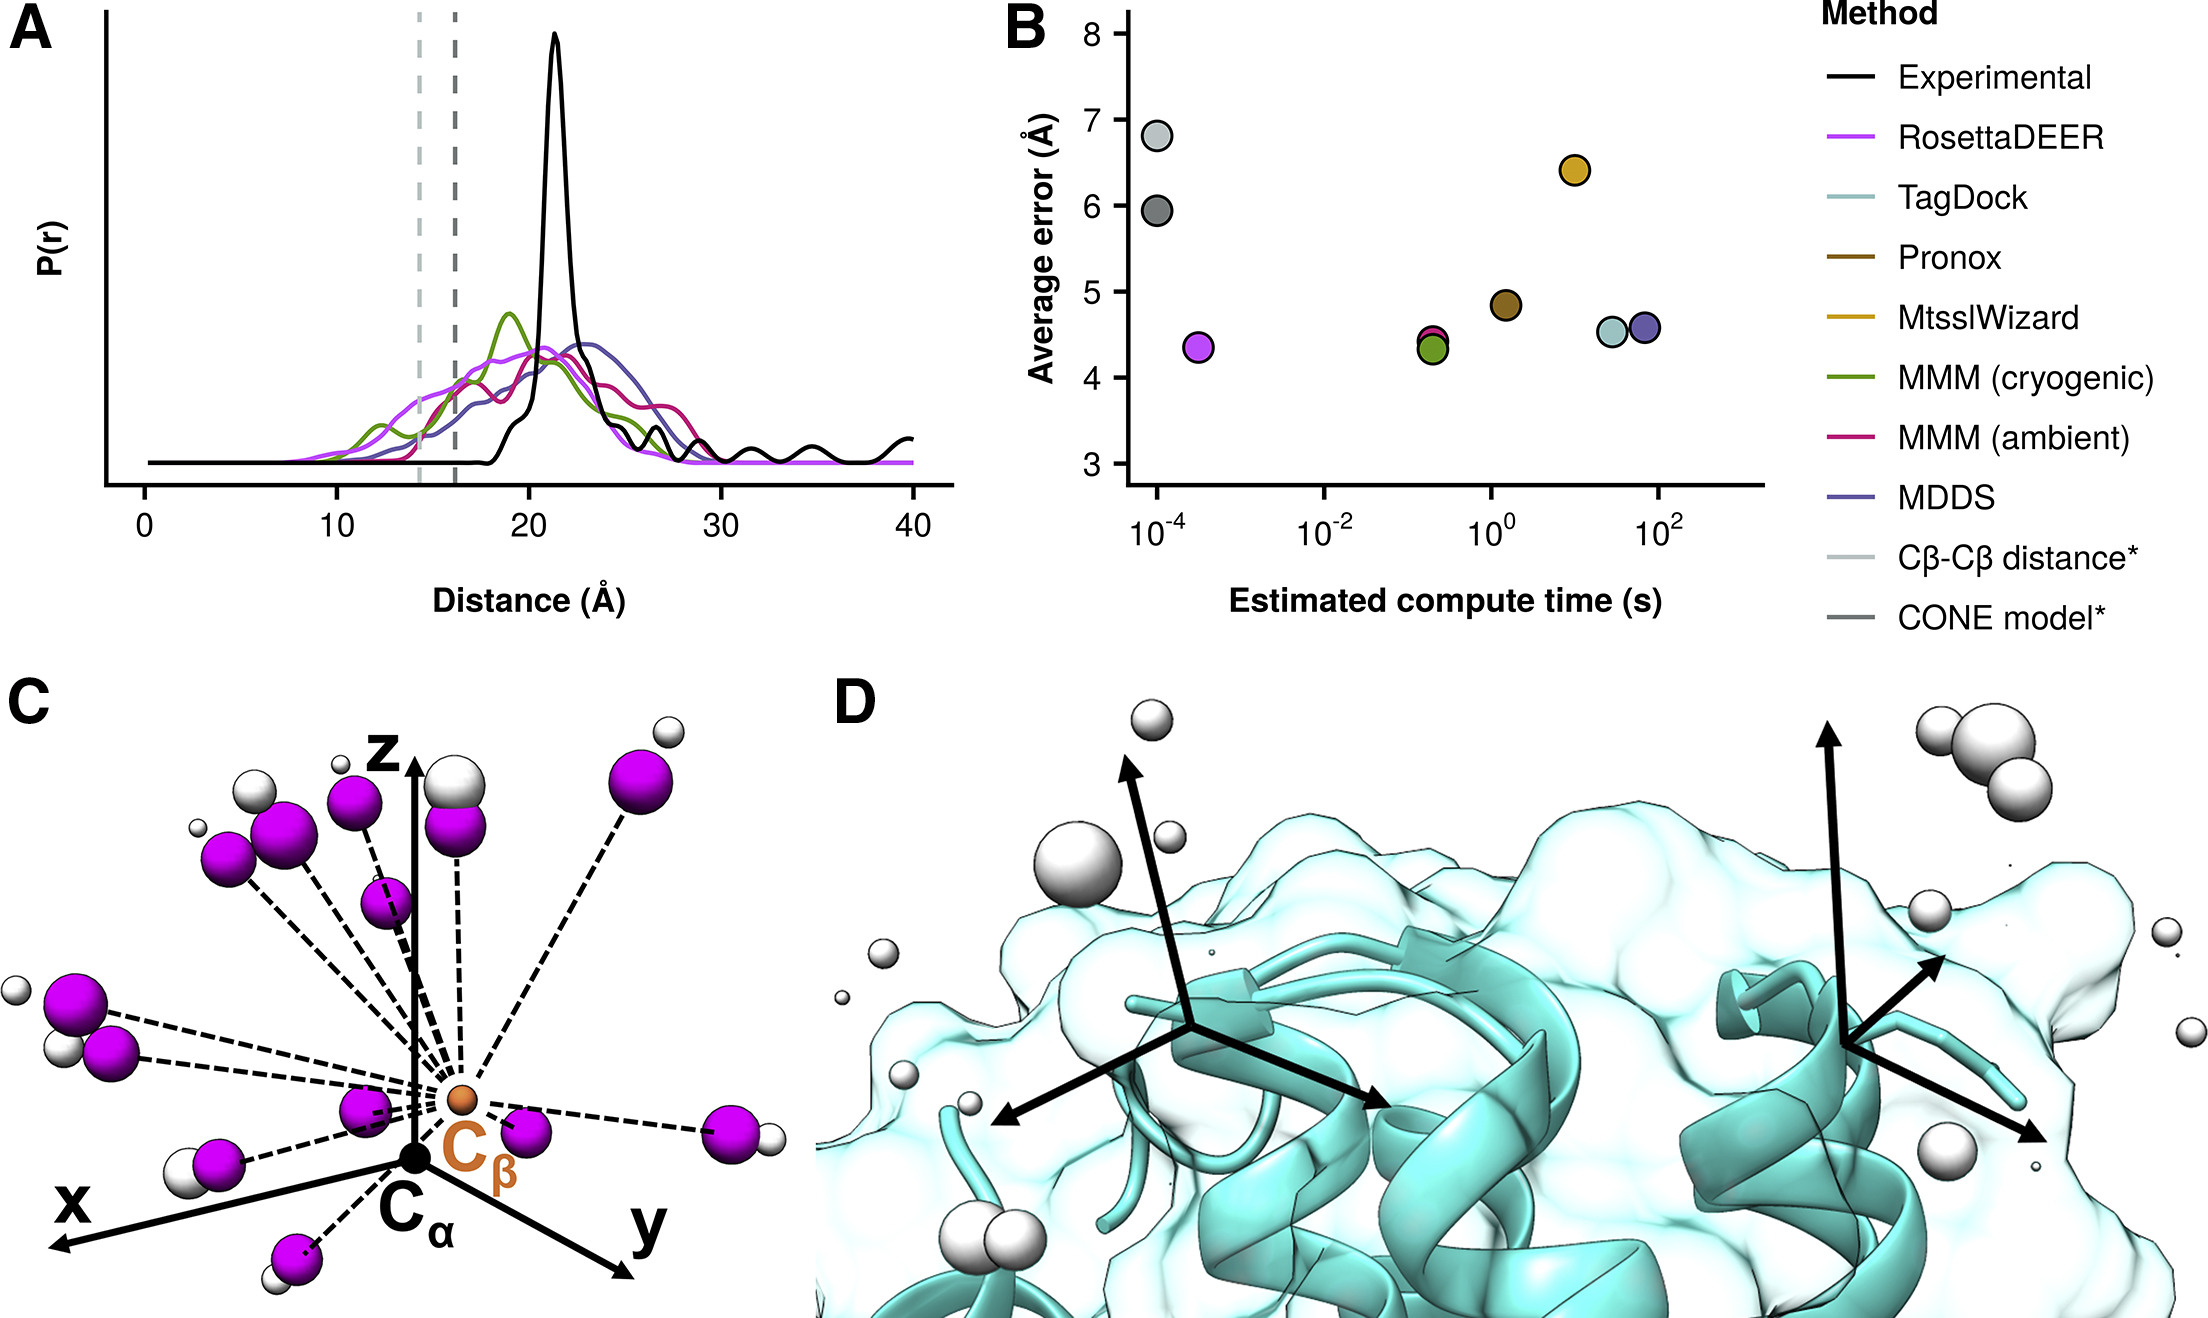
\includegraphics[width=5.5in]{rosettadeer_main_pseudorotamer.jpg}
 \caption[Simulations of distance distributions between nitroxide probes using RosettaDEER.]{Simulations of distance distributions between nitroxide probes using RosettaDEER. (A) An example of an experimentally observed distance distribution in apo Mhp1 51/278, shown in black. Distance distributions were simulated using RosettaDEER, MMM, and MDDS from the occluded Mhp1 structure (PDB: 2JLN). The average distance between $\mathrm{C_{\upbeta}}$ atoms and the average distance calculated using the CONE model shown in light gray and dark gray, respectively. (B) The estimated average time required to simulate distance distributions (*the lower limit of quantification exceeded the $\mathrm{C_{\upbeta}$-$C_{\upbeta}}$ distance compute time). (C) Coarse-grained rotameric ensemble representation of the \gls{mtssl}. Centers of mass, shown in purple, are used for clash evaluation, whereas electron coordinates, shown in gray, serve as measurement coordinates. (D) Distance distributions between residues are simulated by superimposing coordinates, evaluating clashes and measuring all resulting pairwise distances.}
\label{fig:rosettadeer_main_pseudorotamer}
\end{figure}

\subsection{RosettaDEER method description}

The Rosetta rotamer library for the paramagnetic probe \gls{mtssl} \citep*{Alexander2013} served as the basis for the coarse-grained rotameric ensemble used in this study. For each of fifty-four possible rotameric configurations, the unpaired electron was assumed to occupy the nitroxide bond midpoint; it was from these coordinates that distances would be measured. These coordinates were consolidated into a common frame defined by the $\mathrm{C_{\upalpha}}$ atom at the origin, the backbone carbonyl carbon along the Z-axis, and the backbone nitrogen in the Y-Z plane (Figure \ref{fig:rosettadeer_main_pseudorotamer}.C). The remainder of each rotamer was represented by a single pseudo-atom with a radius of \SI{2.4}{\angstrom} that was placed at 87.5\% of the distance between each nitroxide bond midpoint coordinate and an idealized $\mathrm{C_{\upbeta}}$ coordinate; if this pseudo-atom clashed with the protein model, its corresponding electron coordinate was not used for distance measurements. The placement of this pseudo-atom coincides with the center of mass of the nitroxide ring of \gls{mtssl} (all spin-labeled proteins in the PDB are listed in Table \ref{tab:rosettadeer_main_slproteins} and Figure \ref{fig:rosettadeer_supp_sl}). In cases where the steric environment prevented the placement of any coordinates, the van der Waals radius of this pseudo-atom was gradually lowered until at least one rotamer could be accommodated. Distance distributions between two residues reflect all pairwise distance measurements between their respective coordinates after evaluating clashes; we smoothed each of these distance values into gaussian distributions with a \SI{0.5}{\angstrom} standard deviation. The resulting distance distributions were then binned to \SI{0.5}{\angstrom}.

The resulting coordinate frame, which consisted of 54 unweighted coordinates and their positions with respect to protein backbone, did not account for the dynamics of the spin label (e.g. the configurations and positions it preferentially occupies) and was highly redundant, with coordinates often being placed less than \SI{1.0}{\angstrom} apart (Figure \ref{fig:rosettadeer_supp_scheme}). We addressed both issues using a scheme outlined in Figure \ref{fig:rosettadeer_supp_scheme}. Neighboring coordinates were merged using \emph{k}-means clustering to generate a series of coordinate sets ranging from 3 positions to 53 total positions. The weights of these resulting positions were then optimized using 49 previously published experimental distance distributions between 37 residues gathered in T4 Lysozyme \citep*{Islam2013}. During each of half a million iterations, a Monte Carlo Metropolis algorithm randomly modified the weight of a coordinate and either accepted or rejected the change based on the improved agreement with the experimental T4 Lysozyme distance data. This algorithm was carried out on each set of clustered coordinates one thousand times. The resulting set of weights with the best agreement consisted of seventeen coordinates, four of which were fit to be zero. This set was introduced as the default set of coordinates for RosettaDEER and was used for all subsequent experiments described here.

\subsection{Simulation of DEER dipolar coupling decay traces and comparison to experimental values}

Because the simulation of \gls{deer} decay traces has been extensively described \citep*{Hustedt2018, Jeschke2012, Jeschke2006, Marinelli2019}, here we limit our discussion to their generation from distance distributions for the purpose of evaluating protein structural models. The traces simulated by RosettaDEER ($V_{\mathup{sim}}$) are shown in Figure \ref{fig:rosettadeer_supp_alltraces} and reflect coupling between spin labels attached to the same macromolecule ($V_{\mathup{intra}}$), as well as an intermolecular “background” component reflecting coupling between spin labels across different macromolecules:

\begin{equation}\label{eq:rosettadeer_decay_complete}
V_{\mathup{sim}}\left(t_{\mathup{i}},\lambda,k,\vec{r},\vec{w}\right)=\exp\left(-k | t_{\mathup{i}} | \right)*\left(1-\lambda \left(1-V_{\mathup{intra}}\left(t_{\mathup{i}},\vec{r},\vec{w}\right)\right)\right)
\end{equation}

This background is assumed to be homogeneous across three dimensions and is modeled using a slope $k$ and a modulation depth $\lambda$. The simulated distribution consists of a vector of distances $r$ (in nanometers) and their corresponding amplitudes $w$. Simulated traces obtained this way are converted into scores ($S_{\mathup{DEER}}$) by comparing them to the corresponding experimental spectra ($V_{\mathup{exp}}$) using the following cost function:

\begin{equation}\label{eq:rosettadeer_scorefxn}
S_{\mathup{DEER}} = \frac{1}{n} \sum^{n}_{i=1} \left(V_{\mathup{exp}}\left(t_{\mathup{i}}\right)-V_{\mathup{sim}}\left(t_{\mathup{i}},\lambda,k,\vec{r},\vec{w}\right)\right)^{2}
\end{equation}

where $n$ is the number of time points in the data.

To convert a distance distribution into a spectroscopic signal that can be compared to experimental data, RosettaDEER first simulates $V_{\mathup{intra}}$ for each \SI{0.5}{\angstrom} bin $j$ between \SIrange{15}{100}{\angstrom}:

\begin{equation}
V_{\mathup{intra}}\left(t_{\mathup{i}},\vec{r},\vec{w}\right)=\sum^{m}_{j=1}w_{\mathup{j}}*\int_{0}^{\frac{\pi}{2}}\sin \theta \cos \left(\frac{\left(1-3 \cos^2 \theta\right)*\mu_{\mathup{0}} \mu_{\mathup{B}}^{2} g_{\mathup{A}} g_{\mathup{B}} t_{\mathup{i}} }{4 \pi \hslash r_{\mathup{j}}^{3}}\right) \mathup{d} \theta
\label{eq:rosettadeer_kernel}
\end{equation}

where $t$ is the time point of a trace in microseconds, $\mu_{\mathup{B}}$ is the Bohr magneton, $\mu_{\mathup{0}}$ is the vacuum permeability constant, $g_{\mathup{X}}$ is the g-factor of electron $X$, $\theta$ is the angle between the interelectron vector and the bulk magnetic field, and $m$ is the number of distance bins.

Background parameters $k$ and $\lambda$ are then determined and optimized in two stages. Initial values for both parameters were first determined by incrementing $\lambda$ with step size 0.01 and log-transforming \ref{eq:rosettadeer_decay_complete} to determine $k$ using linear regression:

\begin{equation}\label{eq:rosettadeer_logtransform}
\hat{k} = \sum^{n}_{\mathup{i}=1} \left(t_{\mathup{i}}*\ln\left(\frac{V_{\mathup{exp}}\left(t_{\mathup{i}}\right)}{1-\lambda \left(1-V_{\mathup{intra}}\left(t_{\mathup{i}},\vec{r}, \vec{w}\right)\right)}\right)\right) * \left(\sum^{\mathup{n}}_{\mathup{i}=1} t^{2}_{\mathup{i}}\right)^{-1}
\end{equation}

Subsequent attempts to fit simulated intramolecular decay traces were achieved using gradient minimization to solve for $\lambda$ and linear regression to solve for $k$. Convergence was reached when $\lvert \Delta \lambda \rvert < 0.0025$. The iterative strategy used to obtain the initial guess was repeated in cases where $\lambda$ exceeded reasonable values, the lower and upper bounds of which are defined by default as 0.02 and 0.50. This range corresponds to modulation depth values that would ordinarily be obtained from Q-band \gls{deer} on well-labeled double-cysteine mutants without using an arbitrary waveform generator. Deviations from experimentally observed values for these two parameters was found to frequently occur during the initial stages of extended chain \emph{de novo} folding, where simulated distance distributions deviated drastically from experimental values and lead to erroneous background parameter results. 

\subsection{Rosetta model generation and evaluation}\label{sec:rosettadeer_enrichment}

Rosetta models were generated with two approaches to sample a large conformational space but also ensure native-like models at a high density. The native-like models were generated with RosettaCM \citep*{Song2013} using either full-length or truncated native models as inputs. Coverage of a large conformational space was accomplished by \emph{de novo} protein folding. Bax, ExoU, and CDB3 were scored using the \emph{ref2015} energy function \citep*{Alford2017}, and Rhodopsin and Mhp1 were scored using RosettaMembrane \citep*{Yarov-Yarovoy2006}. The transmembrane regions for Rhodopsin and Mhp1 were predicted using OCTOPUS \citep*{Viklund2008}. These models were evaluated using $\mathrm{RMSD_{100SSE}}$, which measures the size-normalized \gls{rmsd} over residues in secondary structures \citep*{Carugo2002}. Enrichment of these models was evaluated as $\log_{10} \frac{TP_{\mathup{P,Score}}*N_{\mathup{Total}}}{P*N_{\mathup{Total}}}$ ⁡where $N_{\mathup{Total}}$ refers to the total number of models being considered, $P$ refers to the proportion of models considered native-like by $\mathrm{C_{\upalpha}}$ $\mathrm{RMSD_{100SSE}}$, and $TP_{\mathup{P,Score}}$ refers to the number of true positives identified in the top $P*N_{\mathup{Total}}$ models by score \citep*{Fischer2015}. We treated the top 10\% of models as native-like ($P$=0.1), thus scaling the metric from -1 (none of the top 10\% of models by $\mathrm{RMSD_{100SSE}}$ were in the top 10\% by score) to 1 (all of the top 10\% of models by $\mathrm{RMSD_{100SSE}}$ were also in the top 10\% by score), with a value of 0 indicating that the number of native-like models found in the top 10\% by score was equal to what is expected by chance.

Oscillation frequencies of decay traces in microseconds for distributions with an average distance $r_{\mathup{avg}}$ (in angstroms) were calculated as $\frac{r_{\mathup{avg}}}{5.2*10^{4}}$  \citep*{Hustedt2018}. Decay traces with fewer than three oscillations were not used to evaluate enrichment as a function of decay trace duration.

\subsection{\emph{De novo} protein structure prediction benchmark}

The protein structure prediction protocol we used largely follows a previously published template \citep*{Ovchinnikov2015} and consists of three stages. In the first stage, 10,000 models were generated using extended chain AbInitio with either RosettaDEER restraints, \gls{cone} model restraints \citep*{Alexander2008}, or no restraints. This protocol relies on the insertion of fragments obtained from a July 2011 copy of the Protein Data Bank and was obtained from the Robetta online server \citep*{Kim2004}; homologous protein structures were excluded from these fragment libraries. The contribution of the RosettaDEER score term was adjusted so that its dynamic range was similar to that of the Rosetta energy function \citep*{Ovchinnikov2015}. Since the proportion of \gls{deer} restraints relative to the protein length was comparable for Bax and ExoU, the impact of the number of restraints on the weight of the score term was not considered \citep*{Weiner2014}. 

Models generated this way were then clustered to a radius of \SI{7.5}{\angstrom} $\mathrm{C_{\upalpha}}$ $\mathrm{RMSD_{100}}$ using Durandal \citep*{Berenger2012}. Each cluster was evaluated by scoring its models using both RosettaDEER and the full-atom Rosetta energy function \citep*{Alford2017}, obtaining the cluster averages for both values, and adding their Z-scores with respect to those of other clusters. After discarding sparsely-populated clusters (smaller than 5\% of the size of the largest cluster), the top ten best-scoring models by combined Z-score were selected from the five best-scoring clusters for subsequent modeling.

An additional 1,200 models were generated from these 50 models using RosettaCM \citep*{Song2013}, which also relies on fragment insertion but ensures that the input model’s topology is retained throughout the modeling process. The scripts were obtained from a recently published refinement protocol \citep*{Park2018}, and no experimental restraints were used. Models generated during this stage were again clustered to \SI{7.5}{\angstrom} $\mathrm{C_{\upalpha}}$ $\mathrm{RMSD_{100}}$ and scored, except only the RosettaDEER score was used to evaluate the quality of these models.

During the third and final stage, models in the best-scoring cluster were minimized using FastRelax \citep*{Conway2014}, which introduces and repacks side chains while performing gradient descent on a full-atom depiction of the entire model. Models generated at this stage were scored exclusively using the native Rosetta energy function, with the lowest-scoring model selected as the output model.

\section{Results}\label{sec:rosettadeer_results}

\subsection{Modeling nitroxide spin labels using RosettaDEER}

A strategy to model proteins using \gls{deer} data must reliably simulate distance distributions between spin-labeled residues. To quantify the computational cost and efficiency of this task, we considered a panel of five proteins, listed in Table \ref{tab:rosettadeer_main_proteins}, where both atomic-detail structures and experimental \gls{deer} data were available \citep*{Altenbach2008, Bleicken2014, Fischer2017, Kazmier2014, Zhou2005}. Distance distributions between residue pairs that have been previously measured experimentally were simulated using a number of methods, and the resulting error was quantified as the difference between the average values of the simulated and experimental distance distributions (example shown in Figure \ref{fig:rosettadeer_main_pseudorotamer}.A). In addition, we measured how rapidly each program calculated these distance distributions (Figure \ref{fig:rosettadeer_main_pseudorotamer}.B). Consistent with previous results \citep*{Fischer2016, Hagelueken2012, Sale2005}, the average values of experimental distance distributions gathered in monomeric proteins, but not the homodimer CDB3, agree more closely with those of simulated distributions than their corresponding $\mathrm{C_{\upbeta}}$-$\mathrm{C_{\upbeta}}$ distances, from which restraints such as the \gls{cone} model are derived \citep*{Alexander2008}. By contrast, none of the methods examined here reliably reproduced the width of the distance distributions. This is likely attributable to oversampling of available conformational space of the spin label, which results from the exclusive use of van der Waals repulsive energies to limit possible rotameric configurations. Finally, the data revealed how simulation times varied substantially between these methods.

These results further illustrate that increasing computational complexity did not lead to more accurate distance distributions. We hypothesized that, for the same reason, decreasing the computational complexity would not lead to less accurate distance distributions. Therefore, RosettaDEER’s design prioritized computational efficiency (see section \ref{sec:rosettadeer_methods}). Rather than measure distances from full-atom rotamers or mobile dummy atoms, RosettaDEER uses a probability density function to capture high-occupancy electron positions that would be explored by \gls{mtssl} and map them onto the protein structure (Figures \ref{fig:rosettadeer_main_pseudorotamer}.C and D). For each of these coordinates, an evaluation of a potential van der Waals overlap was performed between a pseudo-atom representing the nitroxide ring’s center of mass and the rest of the protein. Placing this pseudo-atom at an idealized location, consistent with spin-labeled protein structures in the Protein Databank (Figures \ref{fig:rosettadeer_supp_sl} and Table \ref{tab:rosettadeer_main_slproteins}), reduced the number of atoms for this evaluation to one per rotamer, thus maximizing computational efficiency. Figures \ref{fig:rosettadeer_main_pseudorotamer}.A and B demonstrate that RosettaDEER’s simplified representation of the spin label allows the generation of distance distributions three to five orders of magnitude faster than other approaches but with comparable accuracy.

\begin{figure}[h!]
\centering
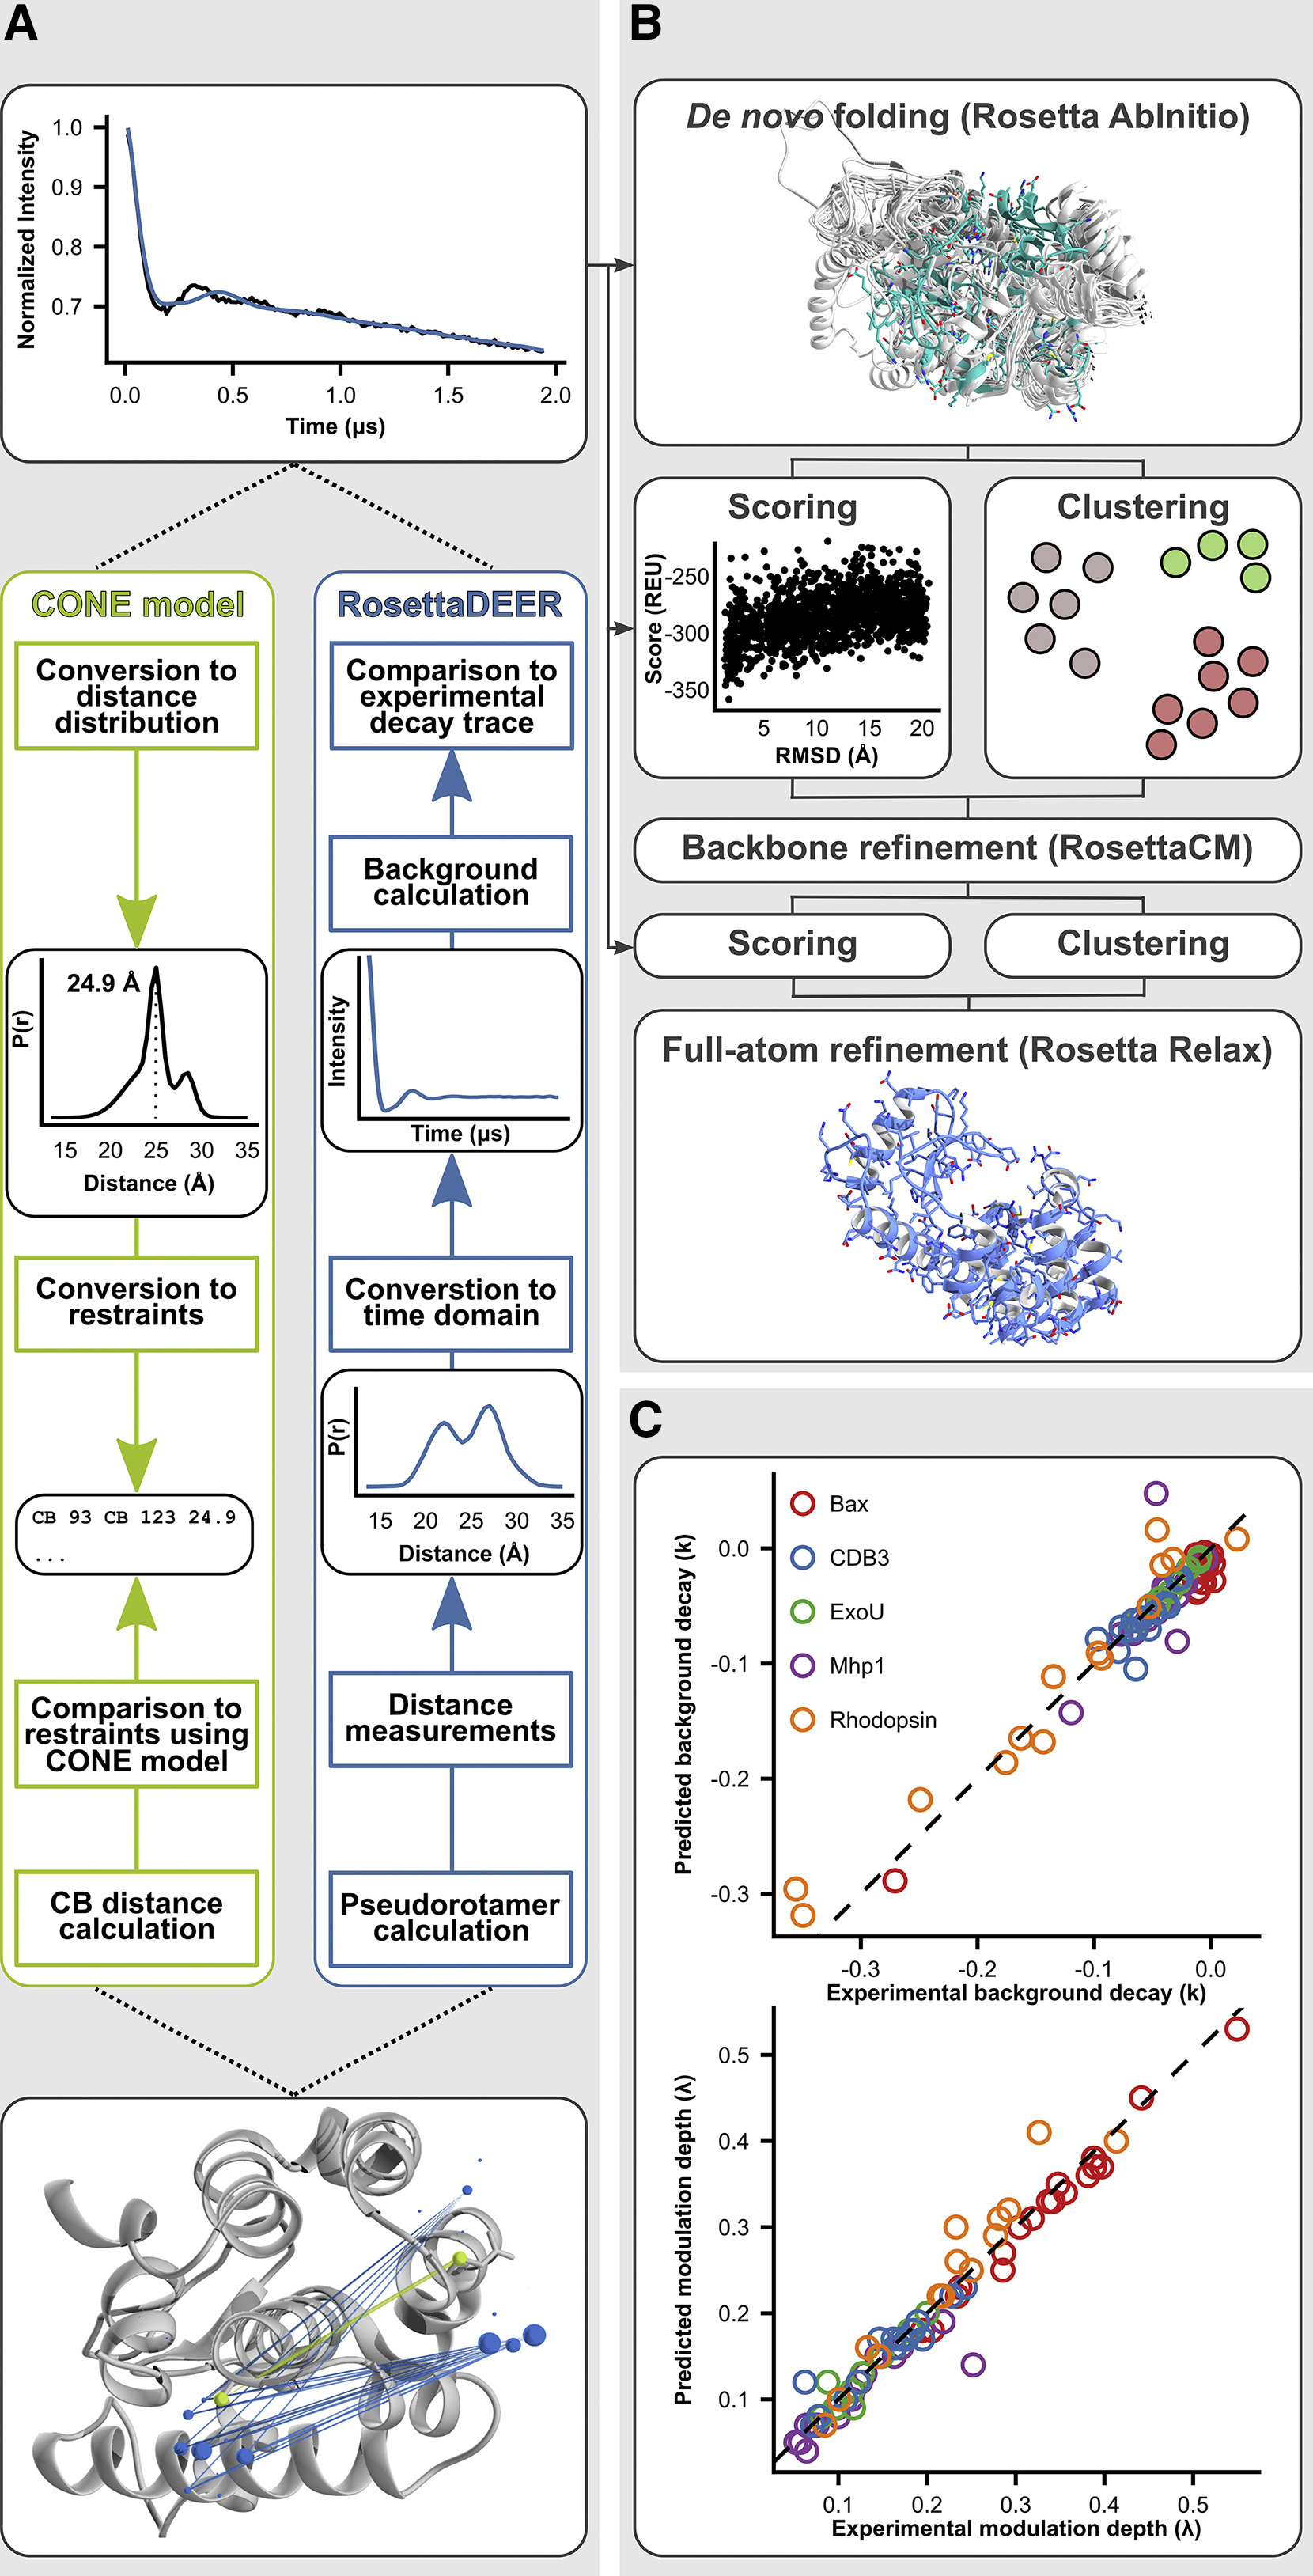
\includegraphics[width=3.25in]{rosettadeer_main_scheme.jpg}
 \caption[RosettaDEER simulations of distance distributions and decay traces.]{RosettaDEER simulations of distance distributions and decay traces. The forward approach taken by RosettaDEER contrasts with the preprocessing required by the CONE model. (A) A flowchart illustrating how both the CONE model and RosettaDEER use experimental \gls{deer} data to model proteins (example shown is T4 lysozyme residues 93 and 123). (B) Incorporation of \gls{deer} experimental restraints into Rosetta structure prediction pipeline. (C) Recovery of experimental background coupling and modulation depth parameter values.}
\label{fig:rosettadeer_main_scheme}
\end{figure}

\subsection{Comparison of simulated with experimental DEER decay traces}

Most existing methods that leverage \gls{deer} experimental data for structural modeling require the primary spectroscopic readout first be processed into a distance distribution. A conventional approach, such as the Rosetta \gls{cone} model, is outlined in Figure \ref{fig:rosettadeer_main_scheme}.A. This involves 1) manually identifying and removing the “background” signal, which corresponds to coupling between spin labels across macromolecules; 2) using Tikhonov regularization to convert the remaining intramolecular signal into a distance distribution; and 3) selecting a single distance value from this distribution to restrain the modeling process. An additional bias is often required to convert these distance data into backbone restraints \citep*{Alexander2008, Alexander2013, Sale2004, Yang2010}.

We reasoned that these preprocessing steps could be avoided by simulating a spectroscopic signal from candidate models for direct comparison to the experimental data. As with other forward approaches to fitting \gls{deer} data \citep*{Hustedt2018, Stein2015}, the steps are as follows: 1) the model is used to generate a distance distribution; 2) this distance distribution is converted into a spectroscopic signal consisting solely of the effect of coupling between spin labels attached to the same macromolecule; and 3) the slope of the “background” coupling and depth of modulation needed to optimally fit the simulated and experimental decay traces is determined.

This final step represents the outstanding challenge in the proposed pipeline, as most modeling programs, including Rosetta, focus on isolated protein structural models. We instead used a two-parameter exponential function to simulate the background coupling ($k$) and modulation depth ($\lambda$) (see Section \ref{sec:rosettadeer_methods}). The values of these parameters were determined by minimizing the sum of the squared residuals. The optimum values obtained strongly correlated with those obtained using DeerAnalysis \citep*{Jeschke2006}, with $r^2$ values exceeding 0.90 for both parameters (Figure \ref{fig:rosettadeer_main_scheme}.C), despite the fact that the inaccuracies in the distance distributions affected the fit (Figure \ref{fig:rosettadeer_supp_alltraces}). In fact, we found that this correspondence correlated less strongly with the goodness-of-fit in the distance domain than it did with the quality of the experimental data in the time domain (Figure \ref{fig:rosettadeer_supp_oscillations}).

\subsection{Enrichment of native-like models using experimental decay traces}

Being able to simulate \gls{deer} traces from candidate structural models without any pre-processing offers the possibility to reframe the problem currently faced by translating the \gls{deer} traces into distance distributions. Whereas methods such as Tikhonov regularization convert individual \gls{deer} traces into distance distributions, RosettaDEER, in conjunction with Monte Carlo modeling, would instead seek to determine the structural model most consistent with both an energy function and the experimental data. To investigate whether unprocessed \gls{deer} traces can be used to discriminate native-like models from incorrectly-folded models, we generated a series of 1000-2000 misfolded models for each of the five proteins in our test set and scored their agreement with experimental \gls{deer} data. In addition, we generated 1000 docked models of the homodimer CDB3 that retained the native fold for the protomer, but not the oligomeric interface. Similarity to the native model was measured by $\mathrm{C_{\upalpha}}$ $\mathrm{RMSD_{100SSE}}$ \citep*{Carugo2002}, which is the size-normalized root means squared deviation across secondary structural elements (Figure \ref{fig:rosettadeer_main_zscores}). RosettaDEER’s effectiveness at this task was measured by the enrichment parameter, which is defined in the Section \ref{sec:rosettadeer_enrichment} section and quantifies a scoring function’s ability to discriminate native-like models from incorrectly-folded models.

\begin{wrapfigure}{ro!}{0.55\textwidth}
    \centering
    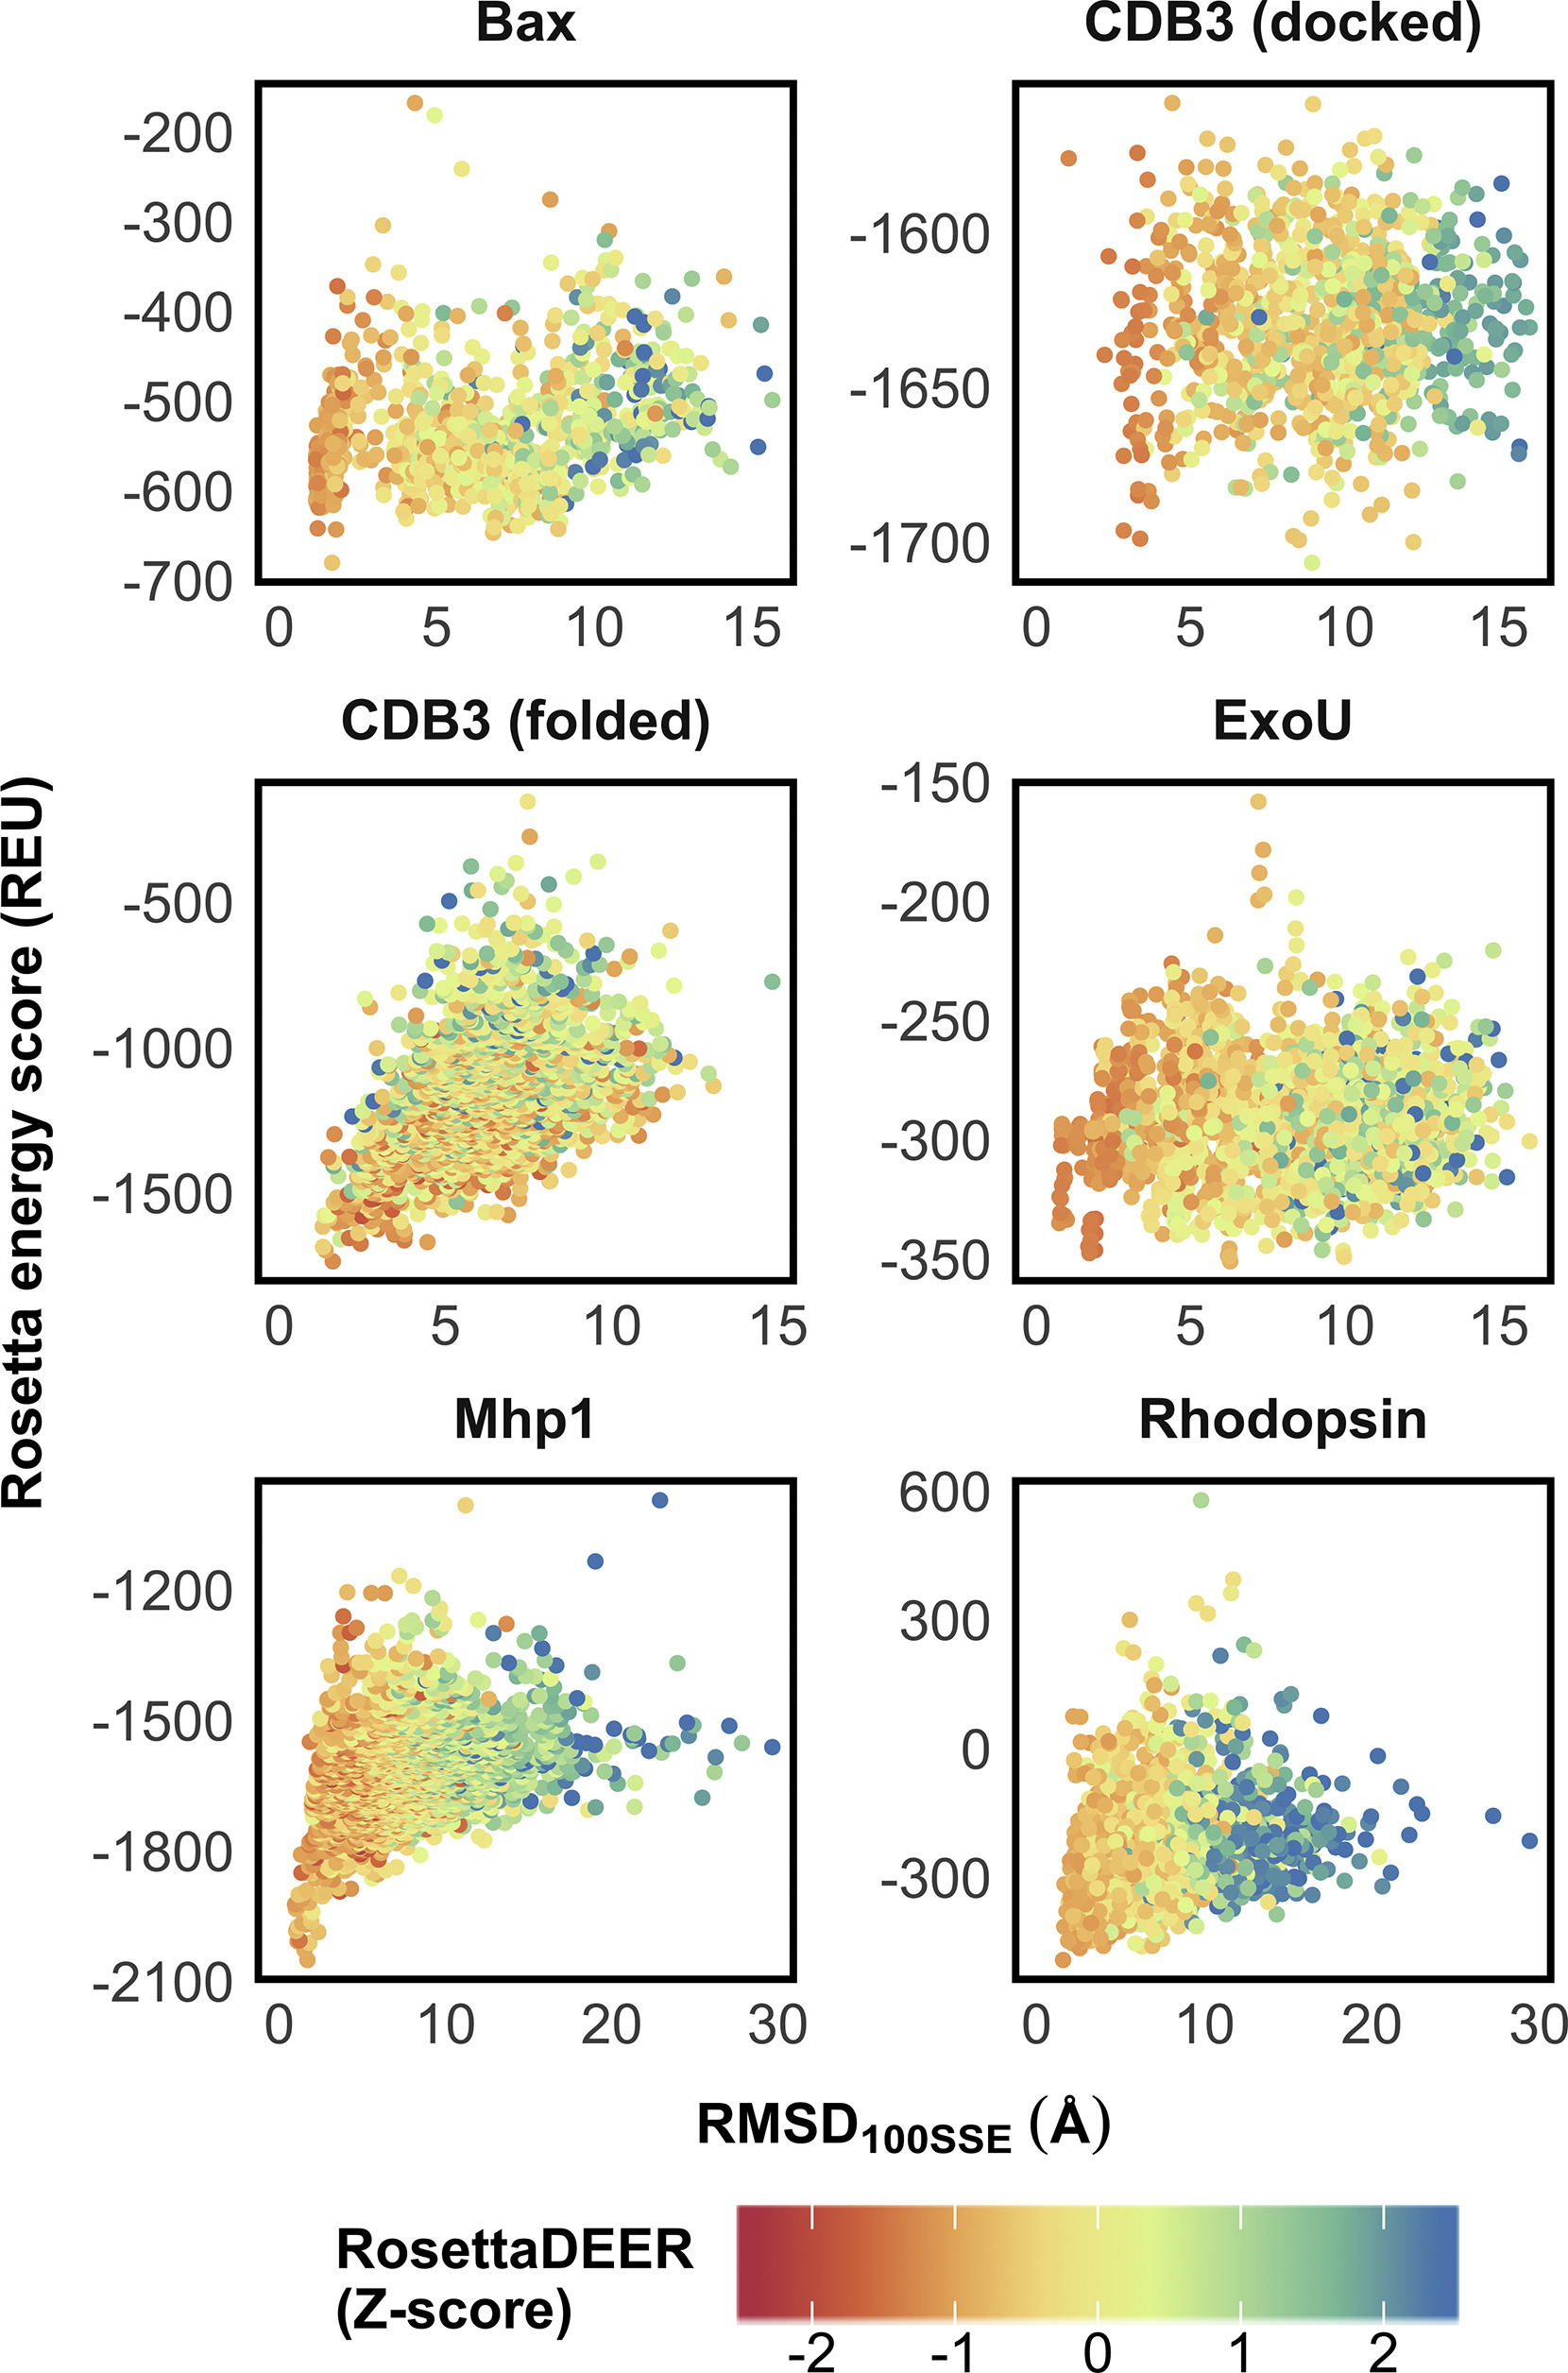
\includegraphics[width=3.25in]{Figures/rosettadeer_main_zscores.jpg}
     \caption[Evaluation of models using \gls{deer} decay traces.]{Evaluation of models using \gls{deer} decay traces. Models with $\mathrm{C_{\upalpha}}$ $\mathrm{RMSD_{100SSE}}$ ranging from \SI{0.5}{\angstrom} to \SI{30.0}{\angstrom} were scored using both the Rosetta energy function and RosettaDEER.}
    \label{fig:rosettadeer_main_zscores}
\end{wrapfigure}

RosettaDEER consistently scored native-like models of the monomeric proteins more favorably than poorly-folded models (Figure \ref{fig:rosettadeer_main_zscores}). This was also observed with correctly-docked models of CDB3. Moreover, it generally outperformed the \gls{cone} model in enriching native-like models (Figure \ref{fig:rosettadeer_supp_oscillation_decoys}). Perhaps unsurprisingly, the simultaneous use of Rosetta’s energy function often improved enrichment, since it overwhelmingly considers short-range interactions and is therefore expected to complement the evaluation of longer ranger, fold-level information provided by \gls{deer} restraints (Figure \ref{fig:rosettadeer_supp_oscillation_decoys}) \citep*{Alford2017}. We note that RosettaDEER could not effectively identify misfolded models of CDB3, which we attribute to the fact that \gls{deer} restraints reflect distances across the center of symmetry, rather than within the protomer. Nevertheless, these results suggest that RosettaDEER’s inability to perfectly recreate the experimental \gls{deer} data did not impede its ability to identify correctly folded models, suggesting that it could be effectively used for structure prediction.



The fact that structural models are scored based on their consistency with the primary spectroscopic data led us to hypothesize that they could be evaluated using lower-quality data than what would be necessary for conversion into precise distance distributions. We were specifically interested in evaluating the importance of the experimental data’s time window, which must undergo roughly 0.8 and 1.6 oscillations for Tikhonov regularization to accurately identify a distance distribution’s average and standard deviation, respectively \citep*{Jeschke2012}. This hypothesis was tested by artificially truncating the experimental data in the time domain and measuring enrichment as a function of how many oscillations were included (see \ref{sec:rosettadeer_methods} and Figure \ref{fig:rosettadeer_supp_oscillation_decoys}). Strikingly, RosettaDEER could enrich native-like models of Bax, ExoU, Rhodopsin, and Mhp1 with highly truncated data ($\mathrm{<0.8}$ oscillations), albeit to a reduced degree. We found that the addition of data in the time domain beyond one oscillation failed to lead to any measurable improvements in enrichment, despite its importance in allowing RosettaDEER to identify the correct background coupling parameters (Figure \ref{fig:rosettadeer_supp_oscillations}). These results suggest that RosettaDEER is more permissive than Tikhonov regularization with respect to the effect of data quality on protein structural modeling.

\subsection{\emph{De novo} folding of Bax and ExoU}\label{sec:rosettadeer_folding_results}

To further illustrate RosettaDEER’s capability to identify native-like models, we folded Bax and ExoU \emph{de novo} using experimental \gls{deer} decay data. These two proteins were chosen because native-like models cannot be identified using the default Rosetta energy function alone (Figures \ref{fig:rosettadeer_main_zscores} and \ref{fig:rosettadeer_supp_oscillation_decoys}). The structure prediction protocol we used is similar to one used to model proteins using other types of sparse data \citep*{Kim2004, Ovchinnikov2015} and is illustrated in Figure \ref{fig:rosettadeer_main_scheme}.B and described in detail in \ref{sec:rosettadeer_methods}. We first generated an initial set of ten thousand models using Rosetta AbInitio folding supplemented by either experimental restraints through RosettaDEER, experimental restraints through the \gls{cone} model \citep*{Alexander2008}, or no restraints. These models were then clustered, and models from the best-scoring clusters were refined and recombined into one thousand two hundred new models without using experimental data. After a second round of clustering, models from the cluster with the best agreement to the experimental data were refined and minimized, and the model with the best Rosetta energy score was returned as the predicted model. 

\begin{wrapfigure}{l}{0.55\textwidth}
    \centering
    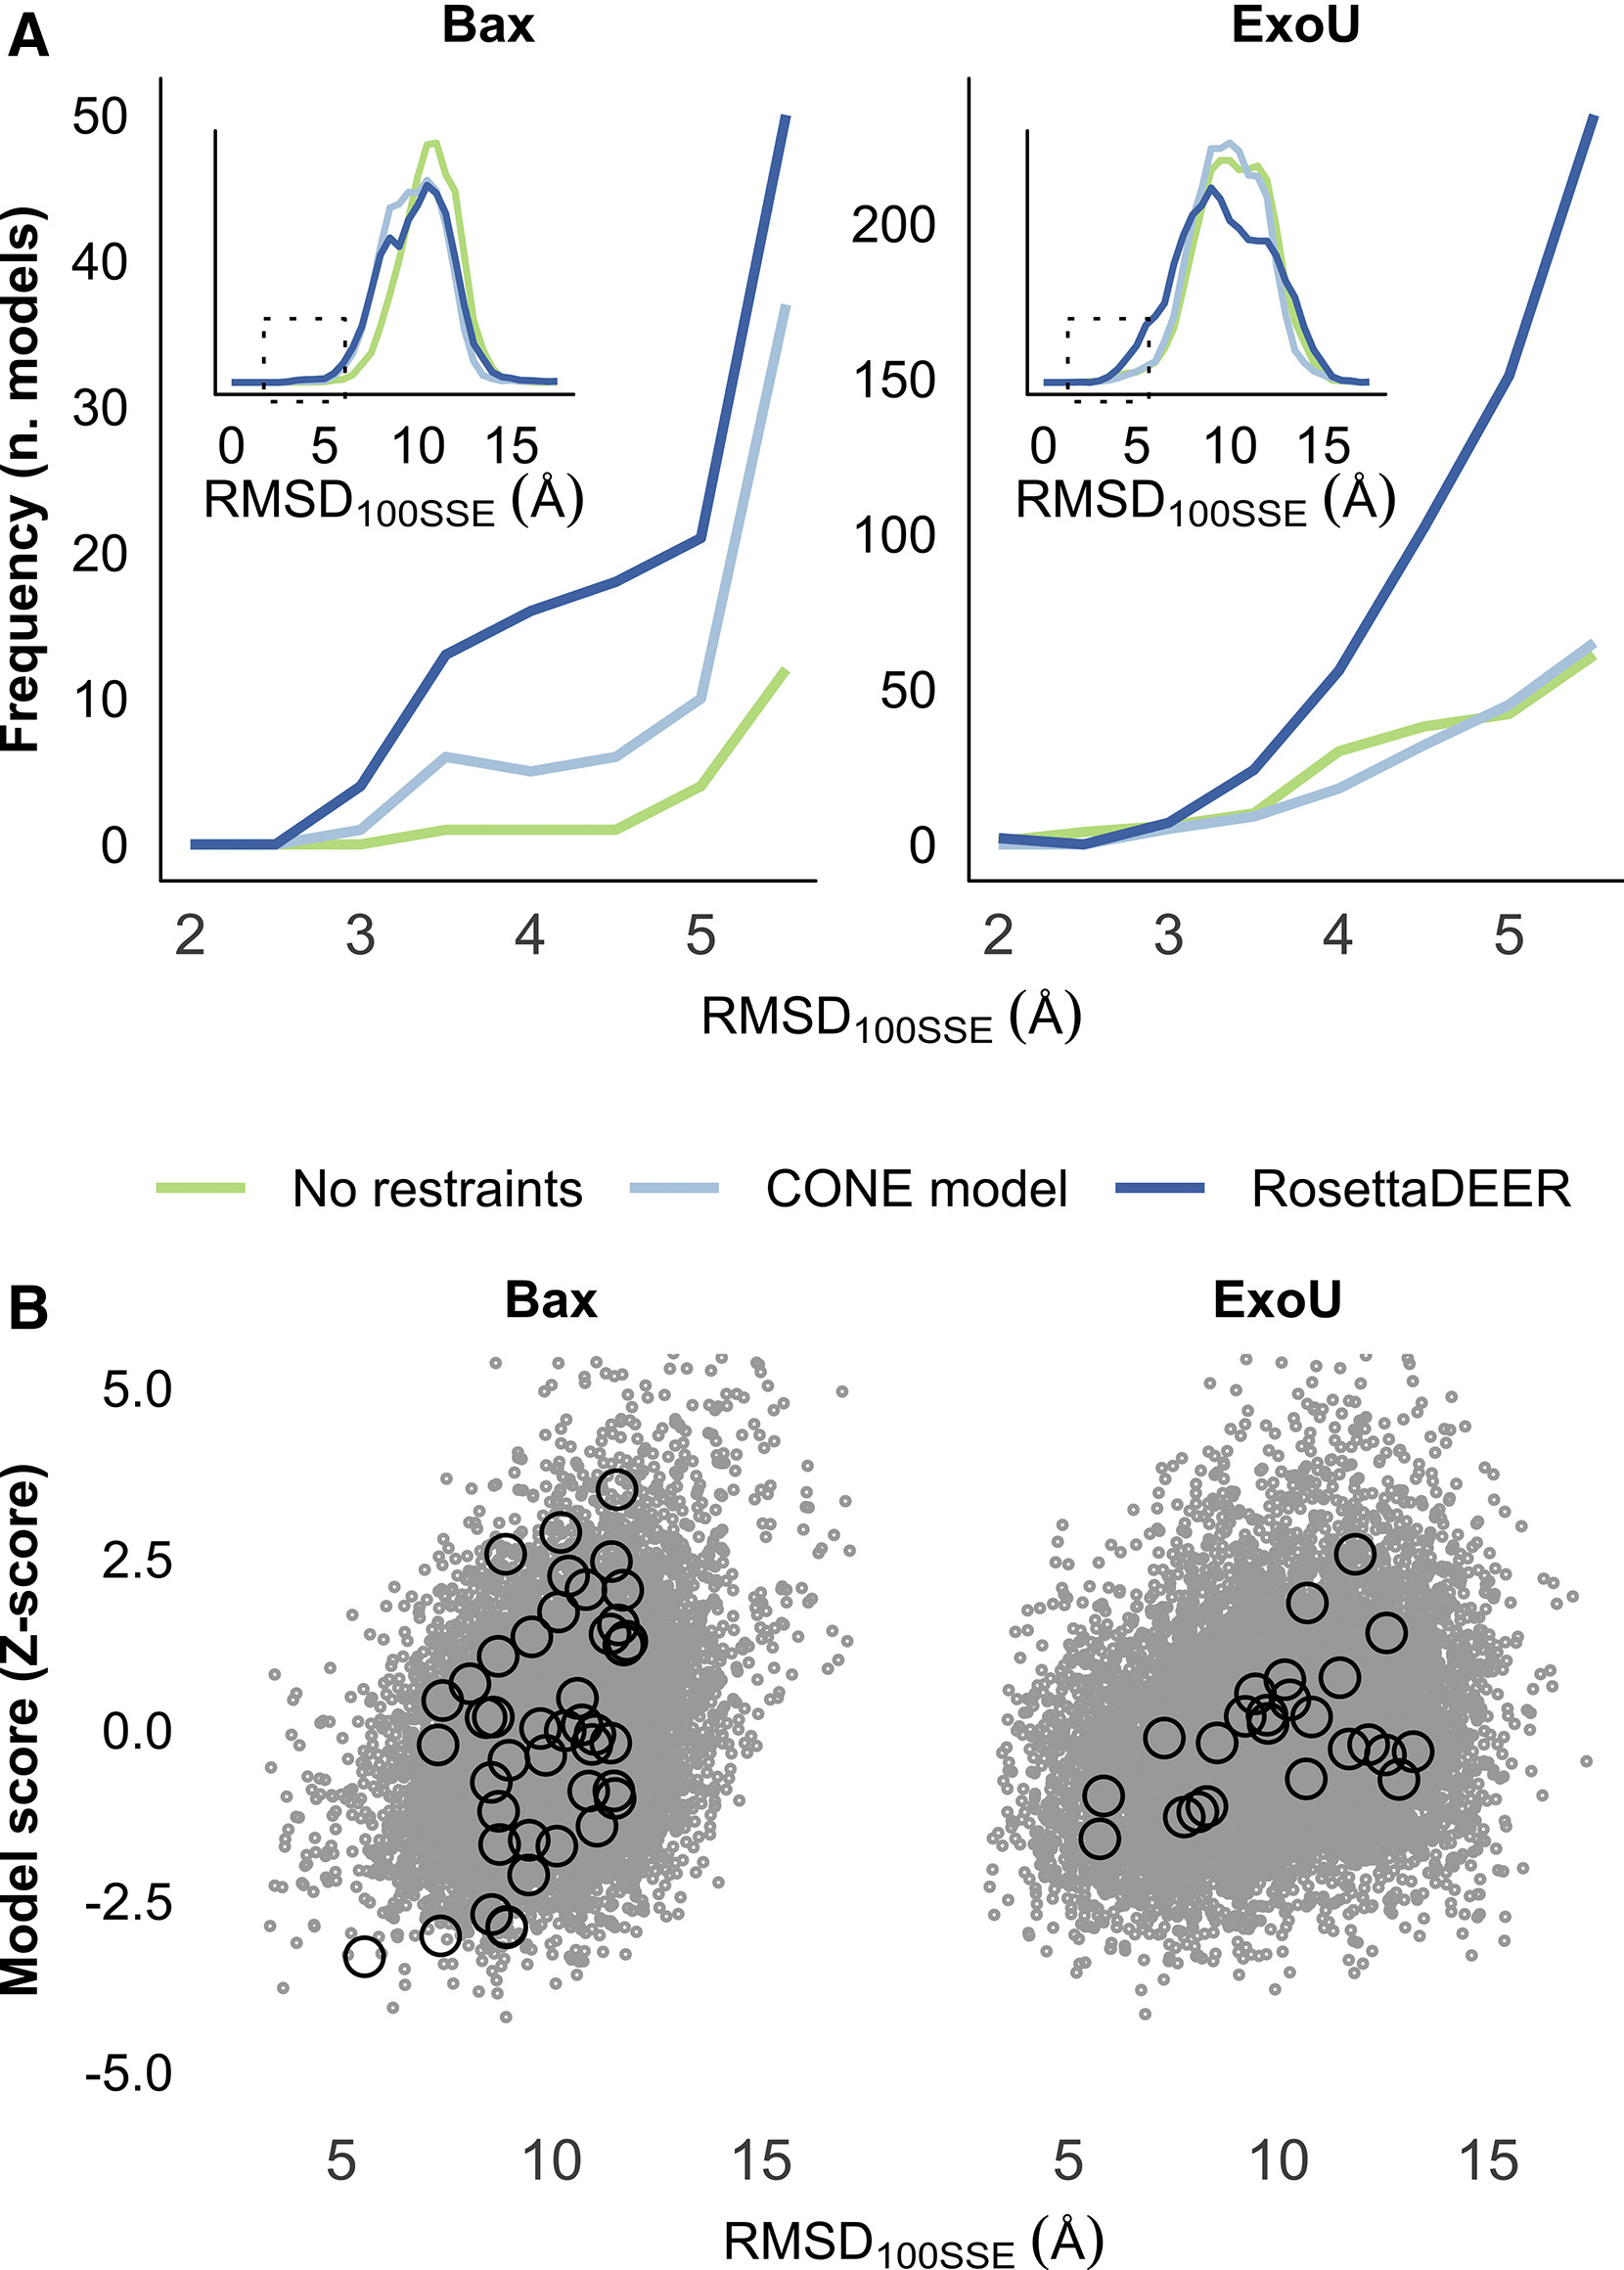
\includegraphics[width=3.25in]{Figures/rosettadeer_main_folding.jpg}
     \caption[Structure prediction of Bax and ExoU using experimental decay data.]{Structure prediction of Bax and ExoU using experimental decay data. (A) \emph{De novo} protein folding of native-like models using \gls{deer} decay restraints with RosettaDEER, $\mathrm{C_{\upbeta}}-\mathrm{C_{\upbeta}}$ distance restraints with the CONE model, or no restraints. Inset: spread of all models generated using these three methods. (B) Accuracy of \emph{de novo} folded models (gray dots) and clusters (black circles) as a function of combined \gls{deer} and Rosetta Z-score.}
    \label{fig:rosettadeer_main_folding}
\end{wrapfigure}

In the absence of experimental restraints, few of the models generated by AbInitio folding resembled the native fold (Figure \ref{fig:rosettadeer_main_folding}.A). Perhaps strikingly, providing \gls{deer} restraints with the \gls{cone} model had no effect on the proportion of native-like models of ExoU generated this way (a measurable improvement was observed when folding Bax). This contrasts with the proportion of native-like models generated using RosettaDEER, which was substantially higher in the case of both proteins.

Although agreement between models and experimental structures loosely correlated with both RosettaDEER score and Rosetta energy score for both proteins, an abundance of incorrectly-folded models obscured this trend (Figure \ref{fig:rosettadeer_main_folding}.B; RosettaDEER and Rosetta energy scores were jointly considered by adding the Z-scores of each). As a result, we were unable to identify native-like models for either Bax of ExoU from score values alone. The ten best-scoring models by these metrics were generally incorrectly folded (\SIrange{5}{10}{\angstrom} $\mathrm{C_{\upalpha}}$ $\mathrm{RMSD_{100SSE}}$) and buried amphipathic features found on the surface of the native model. This shortcoming is typically addressed by clustering, since native-like models are more likely to be found near the centers of large clusters with favorable average scores \citep*{Shortle1998}. We therefore clustered Bax and ExoU models with a radius of \SI{7.5}{\angstrom} and evaluated these clusters by taking the Z-scores of both the average Rosetta energy and RosettaDEER score and adding them together (Figure \ref{fig:rosettadeer_main_folding}.B). In the case of both proteins, this step placed native-like models in the best-scoring clusters. Focusing our attention on the five best-scoring clusters allowed us to discard 85.3\% of the Bax models and 61.3\% of the ExoU models, while retaining a majority of the native-like models in each case.

\begin{wrapfigure}{R}{0.6\textwidth}
    \centering
    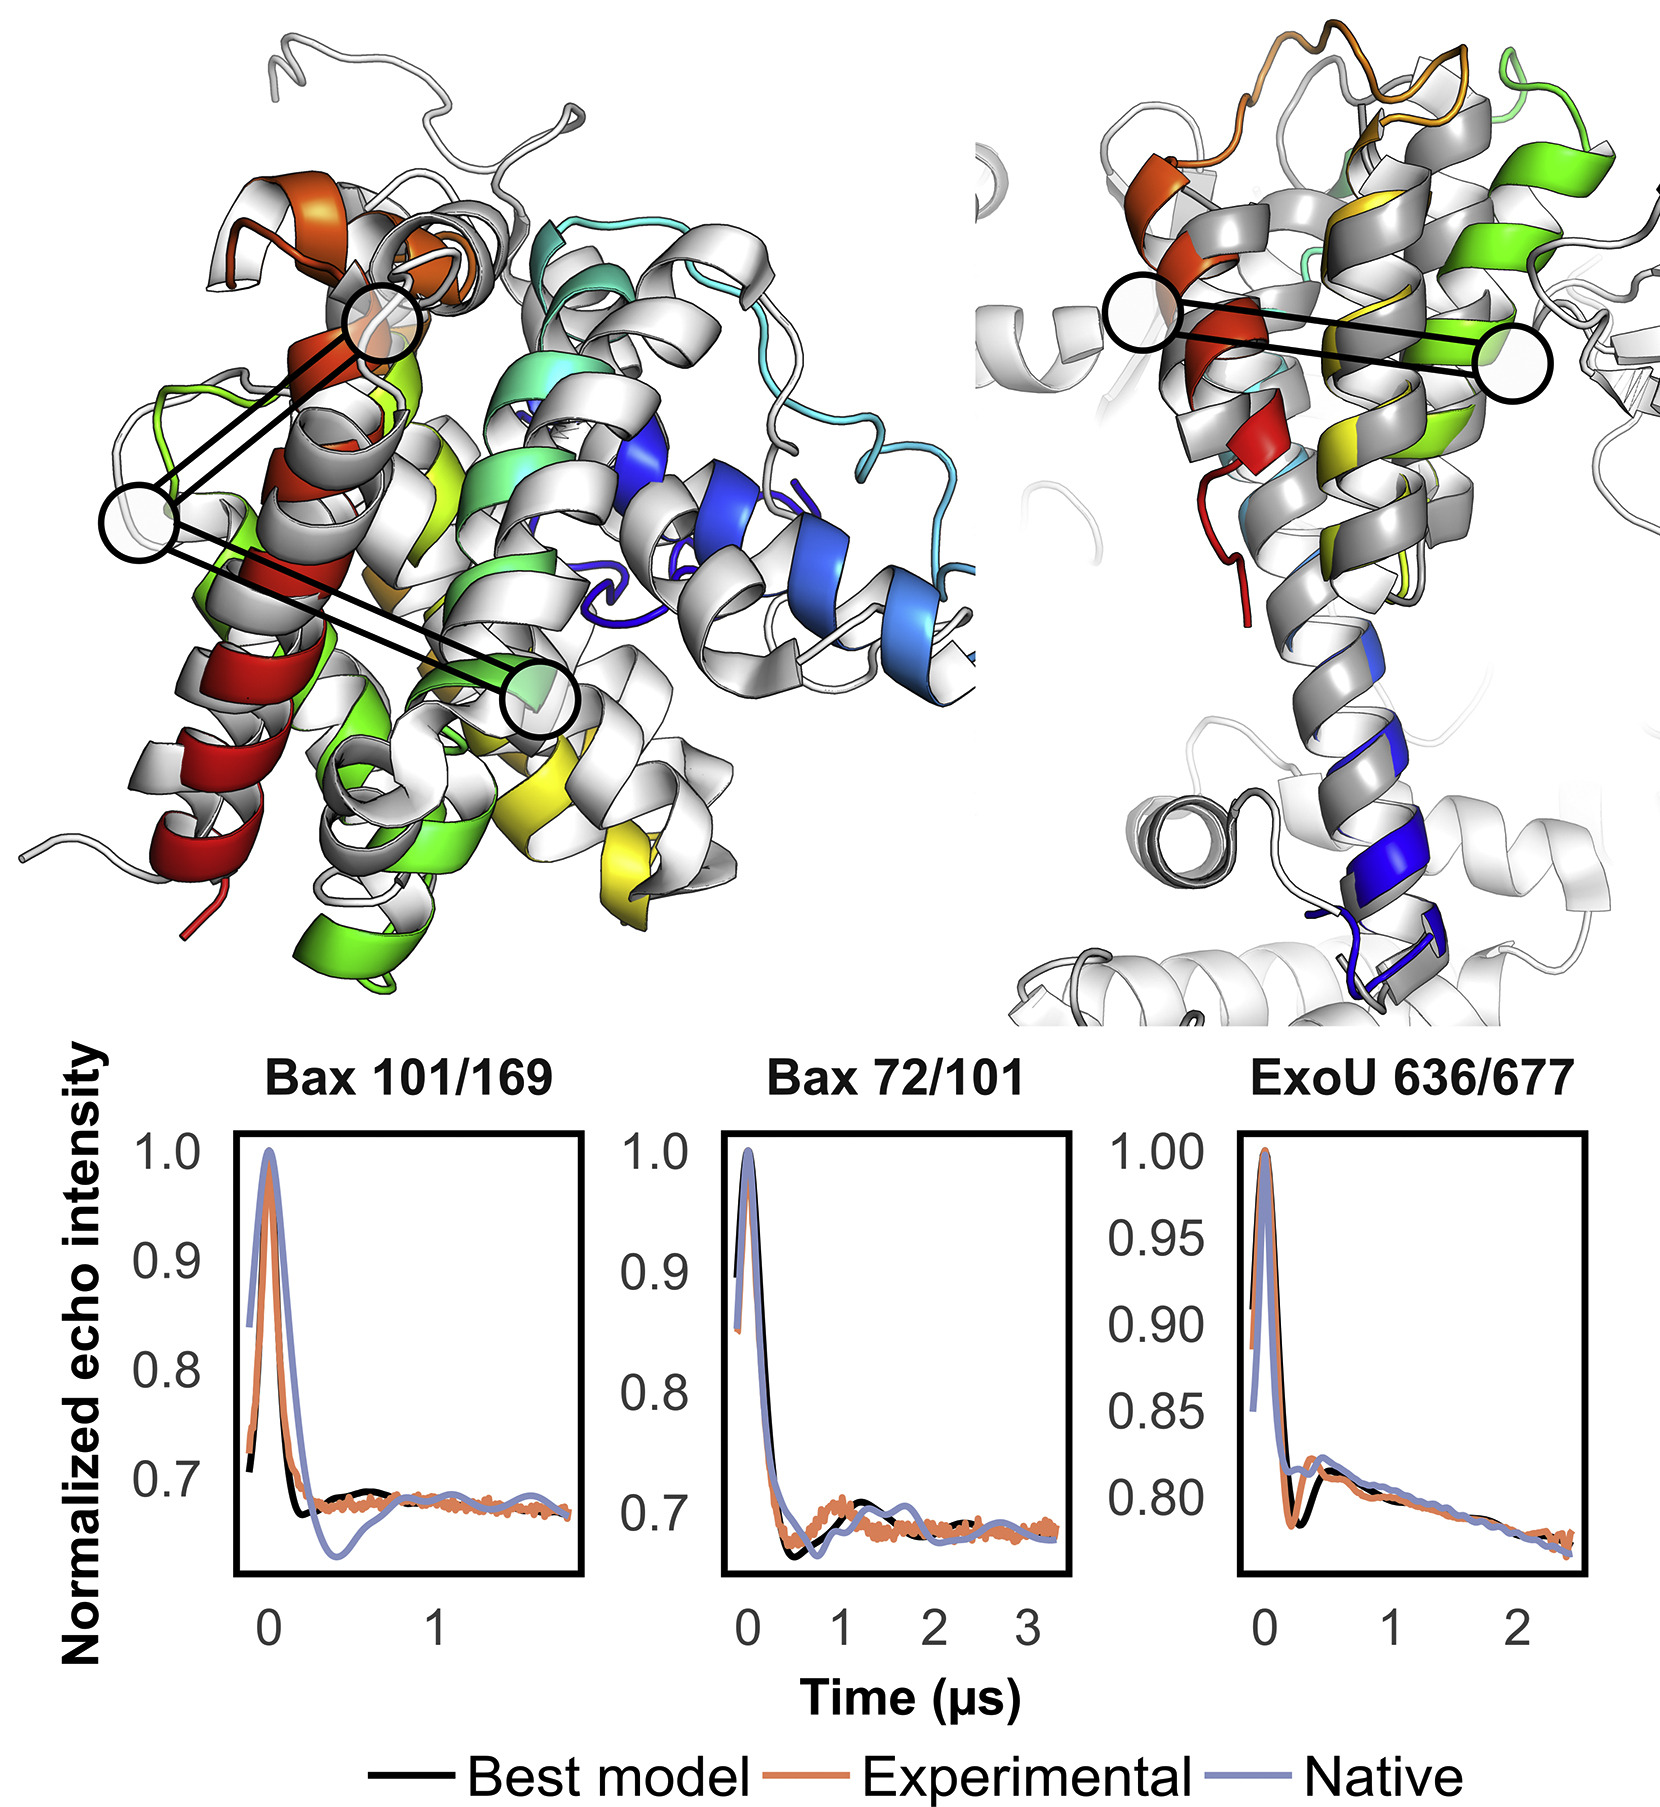
\includegraphics[width=3.25in]{Figures/rosettadeer_main_bestmodels.jpg}
     \caption[Predicted models of Bax and ExoU generated using DEER data.]{Predicted models of Bax and ExoU generated using DEER data. Best-scoring models of Bax and ExoU had an accuracy of \SI{3.2}{\angstrom} and \SI{2.1}{\angstrom} $\mathrm{C_{\upalpha}}$ $\mathrm{RMSD_{100SSE}}$, respectively.(Top) Models were obtained from 10,000 \emph{de novo} folded models, the best-scoring of which were refined into 1200 additional models. Native models shown in white. (Bottom) Example \gls{deer} traces in which the best model outperformed the native. Corresponding residues indicated as circles in (A) and (B).}
    \label{fig:rosettadeer_main_bestmodels}
\end{wrapfigure}

Each cluster at this stage represented a broad population of models that satisfied the \gls{deer} data. To test whether refining models without experimental restraints would reveal the native fold, ten models from each of the top five clusters were refined and recombined using RosettaCM \citep*{Song2013}. This step retained the topology of the input models, but permitted minor backbone rearrangements that allowed misfolded models to optimize away from conformations consistent with the experimental data. As a result, the cluster with the most native-like models after this resampling stage scored the most favorably by RosettaDEER. After minimization of models in this cluster \citep*{Conway2014}, the best-scoring model by Rosetta score for both Bax and ExoU had near-native folds (<\SI{3.5}{\angstrom} $\mathrm{C_{\upalpha}}$ $\mathrm{RMSD_{100SSE}}$; Figure \ref{fig:rosettadeer_main_bestmodels} and \ref{fig:rosettadeer_supp_top3}).

\section{Discussion}

RosettaDEER predicts and refines protein structures by integrating \gls{deer} spectroscopy data and Rosetta computational modeling protocols. The novel aspects of this method are a simplified representation of the commonly used spin label \gls{mtssl} and a strategy to rapidly simulate \gls{deer} decay traces for comparison to uncorrected experimental traces. The robustness of the method was demonstrated by benchmarking every step on five sparse datasets. Despite the simplified spin label representation, the distance distributions simulated by RosettaDEER are comparable to those generated using more computationally complex rotamer library approaches. Moreover, even though simulated spectra fail to perfectly fit experimental \gls{deer} traces, this integrated approach efficiently identifies conformations that simultaneously satisfy the data and the Rosetta energy function. Our findings illustrate how RosettaDEER can complement similar methods that are more computationally intensive but able to use \gls{deer} decay data to perform high-resolution refinement of protein structures \citep*{Marinelli2019}.

The \emph{de novo} folding benchmark with the small soluble proteins ExoU and Bax highlights the success of this strategy. Both proteins possess surface-exposed amphipathic regions that insert into the membrane. Bax transitions from a soluble monomer into a membrane-bound oligomer using its C-terminal helix \citep*{Bleicken2014}, whereas ExoU is hypothesized to move into the membrane using a flexible loop between its two C-terminal helices \citep*{Tessmer2017}. Consistent with previous results \citep*{Fischer2017, Fischer2016}, the Rosetta energy function favored models that packed these substructures in the protein core, leading to incorrectly folded models and lack of correlation between the Rosetta score and model accuracy. As a result, orthogonal experimental data that define the structure are critical to \emph{de novo} folding. Our folding benchmark suggests that RosettaDEER more effectively leverages the experimental data than the $\mathrm{C_{\upbeta}}$-based \gls{cone} model. Moreover, even low-quality data can be used to discriminate native-like from incorrectly-folded models. We appreciate that, for larger proteins, structure determination from \gls{deer} experiments alone would require extensive experimental data. Integrating RosettaDEER with other types of sparse experimental data could therefore reduce the number of \gls{deer} restraints required for accurate modeling.

The strategy of RosettaDEER to predict the structures of these two proteins leverages the experimental data by folding and optimizing protein structures with and without restraints, respectively. The first step leads to a substantial reduction in the search space and a concomitant increase in the number of models that satisfy the restraints, although not all of these models are correctly folded. After clustering the models to remove those that correspond to narrow energy minima, the second step, optimization without restraints, allows clusters with incorrectly folded models to reach energy minima inconsistent with the data. This filtering procedure restores the experimental data’s ability to identify native-like models, since the most native-like models of Bax and ExoU at this stage were not identifiable using the Rosetta energy function. Overall, this protocol decreases both the number of incorrectly-folded structures that fit the data and the conformational search space inherent to the protein folding problem.

Despite its success illustrated here, the current implementation of RosettaDEER assumes that a single protein conformation describes the data. For example, the distance distributions of Mhp1, the most conformationally flexible protein examined in this dataset, were generally more poorly simulated using available methods than those collected in other proteins. Experimental applications of the \gls{deer} technique often focus on monitoring ensembles of protein conformations. They can therefore be effectively complemented by computational methods that interpret this data with the capability to generate multiple models and examine their consistency with sparse experimental data.

\section{Acknowledgements}

The authors would like to thank Dr. Christian Altenbach, Dr. Enrica Bordignon, and Dr. Eric Hustedt for providing experimental data used in this study and Dr. Rocco Moretti, Dr. Axel Fischer, and Dr. Andrew Leaver-Fay for helpful discussions on designing and implementing RosettaDEER. Research was funded by the National Institutes of Health (R01 GM080403, R01 GM073151, R01 GM114234, R01 GM077659, R01 HL122010, and R01 HL144131).